\documentclass[10pt]{academydoc}
\pagestyle{plain}

% Document specific settings/overrides
\renewcommand\lstlistingname{Example}
\lstset{
	tabsize=4,
	basicstyle={\ttfamily\fontsize{8}{9.6}\selectfont},
	frame=single,
	numberbychapter=false,
	captionpos=b
}

% Set Document Details
\doctype{spec} % spec, proc, tb (Specification, Procedure, Technical Bulletin)
\docname{A Common File Format for Look-Up Tables}
\altdocname{A Common File Format for Look-Up Tables}
\docnumber{S-2014-006}
\committeename{Academy Color Encoding System (ACES) Project Committee}
\docdate{March 29, 2016}
\summary{
This document introduces a human-readable text file format for the interchange of color transformations using an XML schema. The XML format supports Look-Up Tables of several types: 1D LUTs, 3D LUTs, and 3by1D LUTs, as well as additional transformation needs such as matrices, range rescaling, and `shaper LUTs'. The document defines a processing model for color transformations where each transformation is defined by a `Node' that operates upon a stream of image pixels. A node contains the data for a transformation, and a sequence of nodes can be specified in which the output of one transform feeds into the input of another node. The XML representation allows saving in a text file both a chain of multiple nodes or a single node representing a unique transform. The format is extensible and self-contained so the XML file may be used as an archival element.
}

% Document Starts Here
\begin{document}

\maketitle

% This file contains the content for the Notices
\prelimsectionformat	% Change formatting to that of "Notices" section
\chapter[Notices]{\uppercase{Notices}}
%% Modify below this line %%

\copyright\the\year{} Academy of Motion Picture Arts and Sciences (A.M.P.A.S.). All rights reserved. This document is provided to individuals and organizations for their own internal use, and may be copied or reproduced in its entirety for such use. This document may not be published, distributed, publicly displayed, or transmitted, in whole or in part, without the express written permission of the Academy.

The accuracy, completeness, adequacy, availability or currency of this document is not warranted or guaranteed. Use of information in this document is at your own risk. The Academy expressly disclaims all warranties, including the warranties of merchantability, fitness for a particular purpose and non-infringement.

Copies of this document may be obtained by contacting the Academy at councilinfo@oscars.org.

``Oscars,'' ``Academy Awards,'' and the Oscar statuette are registered trademarks, and the Oscar statuette a copyrighted property, of the Academy of Motion Picture Arts and Sciences.

% This paragraph is optional.  Comment out if you wish to remove it.
This document is distributed to interested parties for review and comment. A.M.P.A.S. reserves the right to change this document without notice, and readers are advised to check with the Council for the latest version of this document.

% This paragraph is optional.  Comment out if you wish to remove it.
The technology described in this document may be the subject of intellectual property rights (including patent, copyright, trademark or similar such rights) of A.M.P.A.S. or others. A.M.P.A.S. declares that it will not enforce any applicable intellectual property rights owned or controlled by it (other than A.M.P.A.S. trademarks) against any person or entity using the intellectual property to comply with this document.

% This paragraph is optional.  Comment out if you wish to remove it.
Attention is drawn to the possibility that some elements of the technology described in this document, or certain applications of the technology may be the subject of intellectual property rights other than those identified above. A.M.P.A.S. shall not be held responsible for identifying any or all such rights. Recipients of this document are invited to submit notification to A.M.P.A.S. of any such intellectual property of which they are aware.

\vspace{10pt}
These notices must be retained in any copies of any part of this document. \newpage
% This file contains the content for the Revision History and 
\prelimsectionformat	% Change formatting to that of "Notices" section
\chapter{Revision History}
%% Modify below this line %%

\begin{tabularx}{\linewidth}{|l|l|X|}
    \hline
    Version & Date       & Description \\ \hline
    1.0     & 12/19/2014 & Initial Version
    \\ \hline
    1.0.1   & 04/24/2015 & Formatting and typo fixes \\ \hline
            & 03/29/2016 & Remove version number - to use modification date as UID \\ \hline
    &   &   \\ \hline
    &   &   \\ \hline
    &   &   \\ \hline
\end{tabularx}

\vspace{0.25in} % <-- DO NOT REMOVE
\chapter{Related Academy Documents} % <-- DO NOT REMOVE
\begin{tabularx}{\linewidth}{|l|X|}
    \hline
    Document Name & Description \\ \hline
    S-2008-001 & Academy Color Encoding Specification (ACES) \\ \hline
    & \\ \hline
    & \\ \hline
    & \\ \hline
    & \\ \hline
\end{tabularx} \newpage

\tableofcontents \newpage

% This file contains the content for the Acknowledgements
\cleardoublepage
\unnumberedformat	% Change formatting to that of "Acknowledgements" section
\chapter{Acknowledgements} 	% Do not modify section title
%% Modify below this line %%

The Science and Technology Council wishes to acknowledge the following key contributors to the drafting of this document.

\begin{center}
    \begin{tabular}{llll}
        Joseph Goldstone & Jack Holm & Edward Giorgianni & Alex Forsythe \\
        Lars Borg & Harald Brendel & Jim Houston
    \end{tabular}
\end{center}
    
%The Council also wishes to acknowledge the contributions of the members of the \Committeename{} for the development of the concepts and technologies that led to the publication of this document.
%
%\begin{center}
%    \Committeechair{}, Chair, \Committeename{}
%\end{center} \newpage
% This file contains the content for the Introduction
\unnumberedformat	    % Change formatting to that of "Introduction" section
\chapter{Introduction} 	% Do not modify section title
%% Modify below this line %%

The Academy Color Encoding System is a free, open, device-independent color management and image interchange system that can be applied to almost any current or future workflow. It was developed by hundreds of the industry's top scientists, engineers, and end users, working together under the auspices of the Academy of Motion Picture Arts and Sciences.

The primary color encoding in the Academy Color Encoding System (ACES) is the Academy Color Encoding Specification (ACES2065-1).  Academy Color Encoding Specification is standardized in SMPTE ST 2065-1:2012 \cite{SMPTE20651}.  As part of the specification, the encoding primaries and white point were specified as CIE xy chromaticity coordinates to allow for the transformation of ACES2065-1 RGB values to and from other color spaces including CIE XYZ.  Though the CIE xy chromaticity coordinates of encoding red, green, blue and white primaries are only one factor important to unambiguous color interchange\cite{giorgianni}, their specification is required for the calculation of a normalized primary matrix used in color space transformations \cite{smpteRP1997}. The white point used in ACES2065-1 was later adopted for use in other ACES encodings such as ACEScg, ACEScc, ACEScct, etc \cite{ACEScg,ACEScc,ACEScct}. For brevity and inclusiveness, the white point used in the various encodings will be referred to as "the ACES white point" throughout the remainder of this document unless more specificity is required.

The derivation of the ACES white point chromaticity coordinates outlined in this document is intended to help technical users of the ACES system calculate transformations to and from the various ACES encodings in as accurate a manner as possible.  The white point of the ACES encodings does not limit the choice of sources that may be used to photograph or generate source images, nor does it dictate the white point of the reproduction. Using various techniques beyond the scope of this document, the chromaticity of the reproduction of equal ACES2065-1 red, green and blue values (ACES2065-1 \rgbequal) may match the chromaticity of the ACES white point, the display calibration white point, or any other white point preferred for technical or aesthetic reasons

ACES technical documentation is available via ACEScentral.com and oscars.org/aces for product developers wishing to implement ACES concepts and specifications into their products and for workflow/pipeline designers to use ACES concepts and ACES-enabled products for their productions.

% This file contains the content for the Scope
\cleardoublepage
\numberedformat	
\chapter{Scope} 	% Do not modify section title
%% Modify below this line %%

This document describes the derivation of the ACES white point CIE chromaticity coordinates and details of why the chromaticity coordinates were chosen.  This document includes links to an example Python implementation of the derivation and an iPython notebook intended to help readers reproduce the referenced values.

This document is primarily intended for those interested in understanding the details of the technical specification of ACES and the history of its development. The definition of a color space encoding's white point chromaticity coordinates is one important factor in the definition of a color managed system. The white point used in various ACES encodings does not dictate the creative white point of images created or mastered using the ACES system. It exists to enable accurate conversion to and from the other color encodings such as CIE XYZ.  The proper usage of the ACES white point in conversion, mastering, or reproduction are beyond the scope of this document.  For example, the proper usage of the ACES white point in encoding scene colorimetry in ACES2065-1 is detailed in P-2013-001 \cite{idt}.  

% This section contains the content for the References
\numberedformat
\chapter{References}
The following standards, specifications, articles, presentations, and texts are referenced in this text:
%% Modify below this line %%

SMPTE ST 2065-1:2012, Academy Color Encoding Specification (ACES)

SMPTE RP 177:1993, Derivation of Basic Television Color Equations
% This section contains the content for the Terms and Definitions
\numberedformat
\chapter{Terms and Definitions}
The following terms and definitions are used in this document.
%% Modify below this line %%

\term{Academy Color Encoding Specification (ACES)}
RGB color encoding for exchange of image data that have not been color rendered, between and throughout production and postproduction, within the Academy Color Encoding System. ACES is specified in SMPTE ST 2065-1.

\term{ACES RGB relative exposure values}
Relative responses to light of the ACES Reference Image Capture Device, determined by the integrated spectral responsivities of its color channels and the spectral radiances of scene stimuli.

\term{ACES unity neutral}
A triplet of ACES RGB relative exposure values all of which have unity magnitude.

\term{chromatic adaptation}
A process by which the visual mechanism adjusts in response to the radiant energy to which the eyes are exposed.

\term{chromaticity}
A property of a color stimulus defined by the ratios of each tristimulus value of the color stimulus to their sum.

\term{color rendering}
The mapping of image data representing the color-space coordinates of the elements of a scene to output-referred image data representing the color-space coordinates of the elements of a reproduction. Color rendering generally consists of one or more of the following: compensating for differences in the input and output viewing conditions, tone scale and gamut mapping to map the scene colors onto the dynamic range and color gamut of the reproduction, and applying preference adjustments.

\term{color stimulus}
Radiant energy such as that produced by an illumination source, by the reflection of light from a reflective object, or by the transmission of light through a transmissive object, or a combination of these.

\term{focal-plane-referred}
A representation of a captured scene that includes any flare light introduced by the camera’s optical system.

\term{Input Device Transform (IDT)}
A signal-processing transform that maps an image capture system’s representation of an image to ACES RGB relative exposure values.

\term{memory color}
A color sensation derived from memory rather than the immediate perception of a color stimulus.

\term{radiometric linearity}
An attribute of a representation of measured energy in which a change in the amount of measured energy is accompanied by an equal change in the representation of that energy, e.g. a doubling of measured energy is matched by a doubling of the quantity representing that energy.

\term{Reference Input Capture Device (RICD)}
A hypothetical camera, which records an image of a scene directly as ACES RGB relative exposure values.

\term{re-illumination}
An alteration of colors of a captured scene simulating the reflectance of objects in a scene illuminated by an illumination source other than the one under which the scene was captured.

\term{scene adopted white}
A spectral radiance distribution as seen by an image capture or measurement device that is converted to color signals that are considered to be perfectly achromatic and to have an observer adaptive luminance factor of unity; i.e. color signals that are considered to correspond to a perfect white diffuser.

\term{spectral responsivity}
The response of a detection system as a function of wavelength.

\term{spectral sensitivity}
The response of a detector to monochromatic stimuli of equal radiant power.

\term{white balance}
The process of adjusting the RGB signals of an electronic camera system such that equal signals are produced for an object in the scene that is desired to be achromatic \newpage

% This file contains the content for a main section
\regularsectionformat
%% Modify below this line %%
\chapter{Specification}
In the following definitions, \textit{italics} represent a changeable placeholder. \textbf{boldface} represents a required string or character.

\section{String Formats}
ACES system components shall use the following versioning string formats where applicable:

\texttt{\textit{Type.}\textbf{a}\textit{MajorVersionNumber.MinorVersionNumber.PatchVersionNumber}}

or

\texttt{\textit{Type.Name.}\textbf{a}\textit{MajorVersionNumber.MinorVersionNumber.PatchVersionNumber}}

where \texttt{Type} is one of the following:

\begin{listize}
    \item \texttt{IDT} -- ACES Input Transform (a.k.a. ``Input Device Transform'')
    \item \texttt{LMT} -- ACES Look Transform (a.k.a. ``Look Modification Transform'')
    \item \texttt{ODT} -- Output Device Transform
    \item \texttt{RRT} -- Reference Rendering Transform
    \item \texttt{RRTODT} -- ACES Output Transform (concatenated RRT and ODT)
    \item \texttt{InvRRT} -- Inverse Reference Rendering Transform
    \item \texttt{InvODT} -- Inverse Output Device Transform
    \item \texttt{InvRRTODT} -- ACES inverse Output Transform (concatenated RRT and ODT)
    \item \texttt{ACESlib} -- ACES library functions for core transforms, e.g., Tonescales
    \item \texttt{ACEScsc} -- ACES color space conversion transforms
    \item \texttt{ACESutil} -- utility functions provided with the ACES release, e.g., Adjust\_Exposure
\end{listize}

ACES system components are assigned a string that serves as a unique identifier for an ACES System Release. This identifier is constructed using a set of tokens as described in this specification so that it will be more human-readable than a typical Universally Unique Identifier (UUID).

If the \texttt{PatchVersionNumber} is zero, it may be omitted from the versioning string for simplification. If both the \texttt{MinorVersionNumber} and the \texttt{PatchVersionNumber} are zero, they may both be omitted from the versioning string for simplification.

\section{Transform Identifiers}
ACES transforms, expressed as CTL files, are assigned a Transform Identifier.  The Transform Identifier shall be included with all Product Partner implementations intended to match that ACES transform. The Transform Identifier shall be contained in the transform files as metadata or as a comment. For Academy-supplied transforms, the Transform Identifier shall be contained in an XML tag of \texttt{<ACEStransformID>} in the file header.

Product Partner implementation transforms may be intended to match the results of a combined series of ACES CTL transforms, e.g., LMT+RRT+ODT.  In that case, all of the relevant ACES Transform Identifiers shall be included in the implementation Transform. The RRT+ODT combination is a unique case that is covered in \autoref{sec:rrtodt} below.

\section{User-Friendly Names}
ACES Transform Identifiers can be complex and therefore not appropriate for presentation to end users for selection purposes. All transforms shall include ``friendly names'' as metadata within the transform file that software applications may access them for presentation in their user interfaces. For Academy-supplied transforms, the user-friendly name shall be contained in an XML tag of \texttt{<ACESuserName>} in the file header. Recommended friendly names are described in a separate document, ``Academy TB-2014-002, ACES Version 1.0 User Experience Guidelines.''

\section{ACES System Release}
The ACES System Release consists of a variety of ACES core components and ACES vendor-supplied components.

The ACES System Release version shall use the following versioning convention: 

\texttt{\textbf{ACESrelease.a}\textit{MajorVersionNumber.MinorVersionNumber.PatchVersionNumber}}

The ACES System Release patch version number shall be incremented with bug fixes. New patch versions shall not require an update to all transforms.

The ACES System Release minor version number shall be incremented with non-substantive changes to the existing ACES core components. Minor version releases may include new ACES Core Transforms (e.g. new ODTs) and/or roll-ups of minor ODT enhancements/additions or bug fixes. New ACES System Release minor versions shall not require an update to all ACES core and vendor-supplied components.

The ACES System Release major version number shall be incremented with substantive changes to the ACES core components. When the ACES System Release major version number is changed it will require all core and vendor-supplied components be updated to confirm compatibility with the new ACES major version.

The ACES System Release version will not be incremented when ACES vendor-supplied components are updated.

\section{ACES Core Components}
ACES core components include: 

\begin{listize}[-]
	\item ACES Core Transforms
	\item ACES Core Libraries and Utilities
	\item ACES Core File Formats
\end{listize}

\subsection{ACES Core Transforms}
The ACES Core Transforms include the following:

\begin{listize}[-]
	\item The Reference Rendering Transform
	\item Academy-supplied Output Device Transforms
	\item Academy-supplied Look Modification Transforms
	\item Color Space Conversion Transforms
\end{listize}

Transforms such as the RRT and ODTs rely on sub-functions and constants included in separate CTL files, i.e. ACESlib. ACESlib files often contain more than one sub-function or constant. If a change is made to the code of a sub-function that affects the output of a calling transform, the version of the calling transform's Transform Identifier shall be incremented (even if the code in the RRT, ODT, etc. itself may not have changed). For simple additions or modifications to an ACESlib file that do not affect the numerical output of a calling function, the calling function version Transform Identifier will not be incremented. 

Any transform updates that do not change the output of that transform shall not require the Transform Identifier to be incremented - e.g. whitespace changes, modifications to code comments, etc.

Because the results of an ODT depend on the RRT, the version of all ODTs shall be incremented whenever the RRT version is incremented.

\subsubsection{Reference Rendering Transform (RRT)}
The RRT major version number shall match the ACES System Version Major Version number. The RRT Transform Identifier shall use the following versioning convention:

\texttt{\textbf{RRT.a}\textit{ACESmajorVersionNumber.RRTminorVersionNumber.RRTpatchVersionNumber}}

Example Transform Identifiers using this format are: 
\begin{listize}
	\item \texttt{RRT.a1.0.0}
	\item \texttt{RRT.a1}
\end{listize}

\subsubsection{Academy-supplied Output Transforms (ODTs)}
An ODT's major version number shall match the ACES System Version Major Version number. ODT Transform Identifiers shall use the following versioning convention:

\begin{sloppypar}
\texttt{\textbf{ODT}\textit{.Namespace.OutputFormat.\-}\textbf{a}\textit{ACESmajorVersionNumber.\-ODTminor\-Version\-Number.ODTpatchVersion\-Number}}
\end{sloppypar}

\texttt{\textit{Namespace}} identifies the creator of the ODT. The \texttt{\textit{Namespace}} \texttt{Academy} is reserved for Academy-supplied ODTs.

\texttt{\textit{OutputFormat}} fully describes the device and/or output data format of the ODT.

Example Transform Identifiers using this format are:
\begin{listize}
	\item \texttt{ODT.Academy.P3D60\_48nits.a1.0.0}
	\item \texttt{ODT.Academy.Rec709\_D60sim\_100nits\_dim.a1.0.0}
\end{listize}

The Academy provides all ODTs in ACES 1.0, although it is anticipated that vendors will provide ACES-compatible ODTs in the future.

\subsubsection{Academy-supplied Look Modification Transforms (LMTs)}
Academy-supplied LMT's major version number shall match the ACES System Version Major Version number. LMT Transform Identifiers shall use the following versioning convention:

\begin{sloppypar}
\texttt{\textbf{LMT}\textit{.Namespace.Name.\-}\textbf{a}\textit{ACESmajorVersionNumber.\-LMTminorVersionNumber.LMT\-patchVersionNumber}}
\end{sloppypar}

\subsubsection{Color Space Conversion Transforms}
Academy-supplied color space conversions' major version number shall match the ACES System Version Major Version number. Color space conversion Transform Identifiers shall use the following versioning convention:

\begin{sloppypar}
\texttt{\textbf{ACEScsc}\textit{.Name.\-}\textbf{a}\textit{ACESmajorVersionNumber.\-ACEScscMinorVersionNumber.\-ACEScsc\-PatchVersionNumber}}
\end{sloppypar}

\subsection{ACES Core Libraries and Utilities}
Academy-supplied core libraries and utilities' major version number shall match the ACES System Version Major Version number. Core library and utilities Transform Identifiers shall use the following versioning convention:

\begin{sloppypar}
\texttt{\textbf{ACESlib}\textit{.Name.\-}\textbf{a}\textit{ACESmajorVersionNumber.ACESlibMinorVersionNumber.ACESlib\-Patch\-Version\-Number}}
\end{sloppypar}

\begin{sloppypar}
\texttt{\textbf{ACESutil}\textit{.Name.\-}\textbf{a}\textit{ACESmajorVersionNumber.ACESutilMinorVersionNumber.ACES\-utilPatchVersionNumber}}
\end{sloppypar}


\subsection{ACES Core File Formats}
The ACES Core File Formats include the following:

\begin{listize}[-]
	\item SMPTE ST 268:2014 (DPX)
	\item SMPTE ST 2065-4:2013 (ACES Image Container File Layout)
	\item ACES Clip-level Metadata File (clip-level metadata sidecar)
	\item Academy-ASC Common LUT Format File (CLF)
\end{listize}

The SMPTE standard file formats are versioned according to SMPTE conventions.

ACES Clip Metadata files and Academy-ASC Common LUT Format files shall contain a metadata field that identifies the ACES System Version Number with which they conform, and the required Transform Identifiers of the transforms referenced therein (see ``Academy TB-2014-009'' and ``Academy S-2014-006'' for additional details).

\section{ACES Vendor-supplied components}
Certain ACES components, such as Input Transforms and concatenated RRT/ODTs, are shipped by ACES Product Partners and therefore are not constrained to ACES System release schedules. Other ACES components, such as ODTs and LMTs, are likely to be vendor-supplied in the future. Nonetheless, the versioning and naming requirements are the same as for ACES core components in that they must be identified as being compatible with a given ACES major system release.

To enable easier reading and parsing of Transform Identifiers, the sub-strings used for \texttt{\textit{NameSpace}} and \texttt{\textit{DeviceName}} should not contain spaces or periods and should also be limited to the ASCII character set.

\subsection{Input Transforms (IDTs)}

\texttt{\textbf{IDT}\textit{.NameSpace.DeviceName.}\textbf{a}\textit{ACESmajorVersionNumber.}\textbf{v}\textit{IDTversionNumber}}

The creator of the IDT shall be identified using the \texttt{\textit{NameSpace}}. When the creator of the transforms is the manufacturer of the camera then the device is not required to repeat the manufacturer name.  If the IDT creator is not the camera manufacturer, then the manufacturer name shall be prepended to the \texttt{\textit{DeviceName}}.

Example IDT Transform Identifiers using this format are: 
\begin{listize}
	\item \texttt{IDT.Sony.F65.a1.v1}
	\item \texttt{IDT.Arri.AlexaEI100T.a1.v2}
	\item \texttt{IDT.Dolby.ArriAlexa.a1.v1}
\end{listize}

\subsection{Look Transforms (LMTs)}

\texttt{\textbf{LMT}\textit{.Namespace.Name.}\textbf{a}\textit{ACESmajorVersionNumber.}\textbf{v}\textit{LMTversionNumber}}

The creator of the LMT shall be identified using the \texttt{\textit{NameSpace}}. The \texttt{\textit{NameSpace}} \texttt{Academy} is reserved for Academy-supplied LMTs. The \texttt{\textit{Name}} shall identify the purpose the LMT serves.

Example LMT Transform Identifiers using this format are: 
\begin{listize}
	\item \texttt{LMT.Academy.ACES\_0\_7\_1.a1.v1} (Academy-supplied v0.7.1 backwards-compatible transform)
	\item \texttt{LMT.ACME.BleachBypass.a1.v1} (ACME Transform, Inc.-supplied bleach bypass LMT compatible with ACES Version 1.0, in the Academy-ASC Common LUT Format)
\end{listize}

\subsection{Output Transforms (ODTs)}

\texttt{\textbf{ODT}\textit{.Namespace.OutputFormat.}\textbf{a}\textit{ACESmajorVersionNumber.}\textbf{v}\textit{ODTversionNumber}}

\texttt{\textit{NameSpace}} shall identify the creator of the ODT. The \texttt{\textit{NameSpace}} \texttt{Academy} is reserved for Academy-supplied ODTs. 

\texttt{\textit{OutputFormat}} fully describes the device and/or output data format of the ODT.

Example Transform Identifiers using this format are:
\begin{listize}
	\item \texttt{ODT.ACME.P3D60ProjectorSomeSpecialCalibration.a1.v1}
	\item \texttt{ODT.ACME.Rec709\_D60sim\_100nits\_dim.a1.v10}
\end{listize}

\subsection{Concatenated Reference Rendering Transform/Output Transforms (RRT/ODTs)} \label{sec:rrtodt}

\texttt{\textbf{RRTODT}\textit{.Namespace.OutputFormat.}\textbf{a}\textit{ACESmajorVersionNumber.}\textbf{v}\textit{ODTversionNumber}}

\texttt{\textit{Namespace}} shall identify the creator of the concatenated RRT/ODT. The \texttt{\textit{Namespace}} \texttt{Academy} is reserved for Academy-supplied concatenated RRT/ODTs.

\texttt{\textit{OutputFormat}} fully describes the device and/or output data format of the concatenated RRT/ODT, and should use the \texttt{\textit{OutputFormat}} associated with the ODT used in the concatenated transform. 

Example Transform Identifiers using this format are: 
\begin{listize}
	\item \texttt{RRTODT.ACME.P3d60Projector.a1.v1}
	\item \texttt{RRTODT.ACME.Rec709\_D60sim\_100nits\_dim.a1.v1}
	\item \texttt{RRTODT.ACME.P3D60ProjectorSomeSpecialCalibration.a1.v1}
	\item \texttt{RRTODT.ACME.Rec709\_d60sim\_8000nits.a1.v1}
\end{listize}

\section{Implementation Version Reporting}
ACES implementations shall report the version of the ACES System in use to at least the Minor Version Number.  Reporting of the Patch Version Number is optional. For more details, refer to ``Academy TB-2014-002.''

\section{ACES Pre-release Versions}
Pre-release versions of ACES, i.e., versions prior to Version 1.0, shall use the following version string format:

\texttt{\textbf{aPR}\textit{majorVersionNumber.MinorVersionNumber.PatchVersionNumber}}

Example:
\begin{listize}
	\item \texttt{ACESrelease.aPR0.7.1}
\end{listize}

The ``\texttt{\textbf{aPR}}'' designation indicates a version of ACES prior to the Version 1.0 release and the use of any transforms with this designation is deprecated.
% This file contains the content for a main section
\regularsectionformat
%% Modify below this line %%
\chapter{Conventions and Constraints}
\label{sec:conventions}

Some characteristics of the XML format are constrained to improve interoperability and interchange between the different systems that use LUTs. These constraints may be loosened over time as implementations and computer capabilities improve. It is desirable that implementations support the full capabilities of the specification, but it is recognized that portability and ease of implementation are needed in current deployments.

The constraints listed in this section serve to identify key parameters that an implementation reader must be able to use.

Among these agreed upon conventions are:

This specification uses the \texttt{ProcessList} as the root node in an XML file.  Storing multiple \texttt{ProcessList}s in a file requires definition of a higher-level XML schema for that purpose which is not addressed here.

Matrices are 3x3, 3x4, or 4x4. 3x4 matrices provide an offset value in the 4th column to be added to the results of the previous 3 columns.  

3-component processing is the normal mode of operation.  1-component processing is possible with only a \texttt{LUT1D} node and if needed a \texttt{Range} node, but is not a required feature.

\texttt{LUT3D}s have the same dimension on all axes (i.e. \texttt{Array} dimensions are of the form "n n n 3").  A \texttt{LUT3D} with axial dimensions greater than 128x128x128 should be avoided.

Software applications are required to support two 3DLUT interpolation types: ``trilinear'' and ``tetrahedral''.  ``Linear'' interpolation is required as a default for 1DLUTs.

\texttt{LUT1D} lengths should be limited to at most 65536 entries.

As a general principle, the LUT output values should make explicit the clipping behavior for values outside of the region of interest. The \texttt{Range} node can be used for clamping of values.

Supported bit depth values are ``\texttt{8i}'', ``\texttt{10i}'', ``\texttt{12i}'', ``\texttt{16i}'', ``\texttt{16f}'' and ``\texttt{32f}''.

``\texttt{12i}'' is present for processing of digital cinema 12-bit DCDMs. ``\texttt{16f}'' are half floats as described in IEEE 754-1985. All integer values are unsigned ints. ``\texttt{32f}'' LUTs should never be fully enumerated.
 
\begin{figure}[htbp]
\begin{center}
    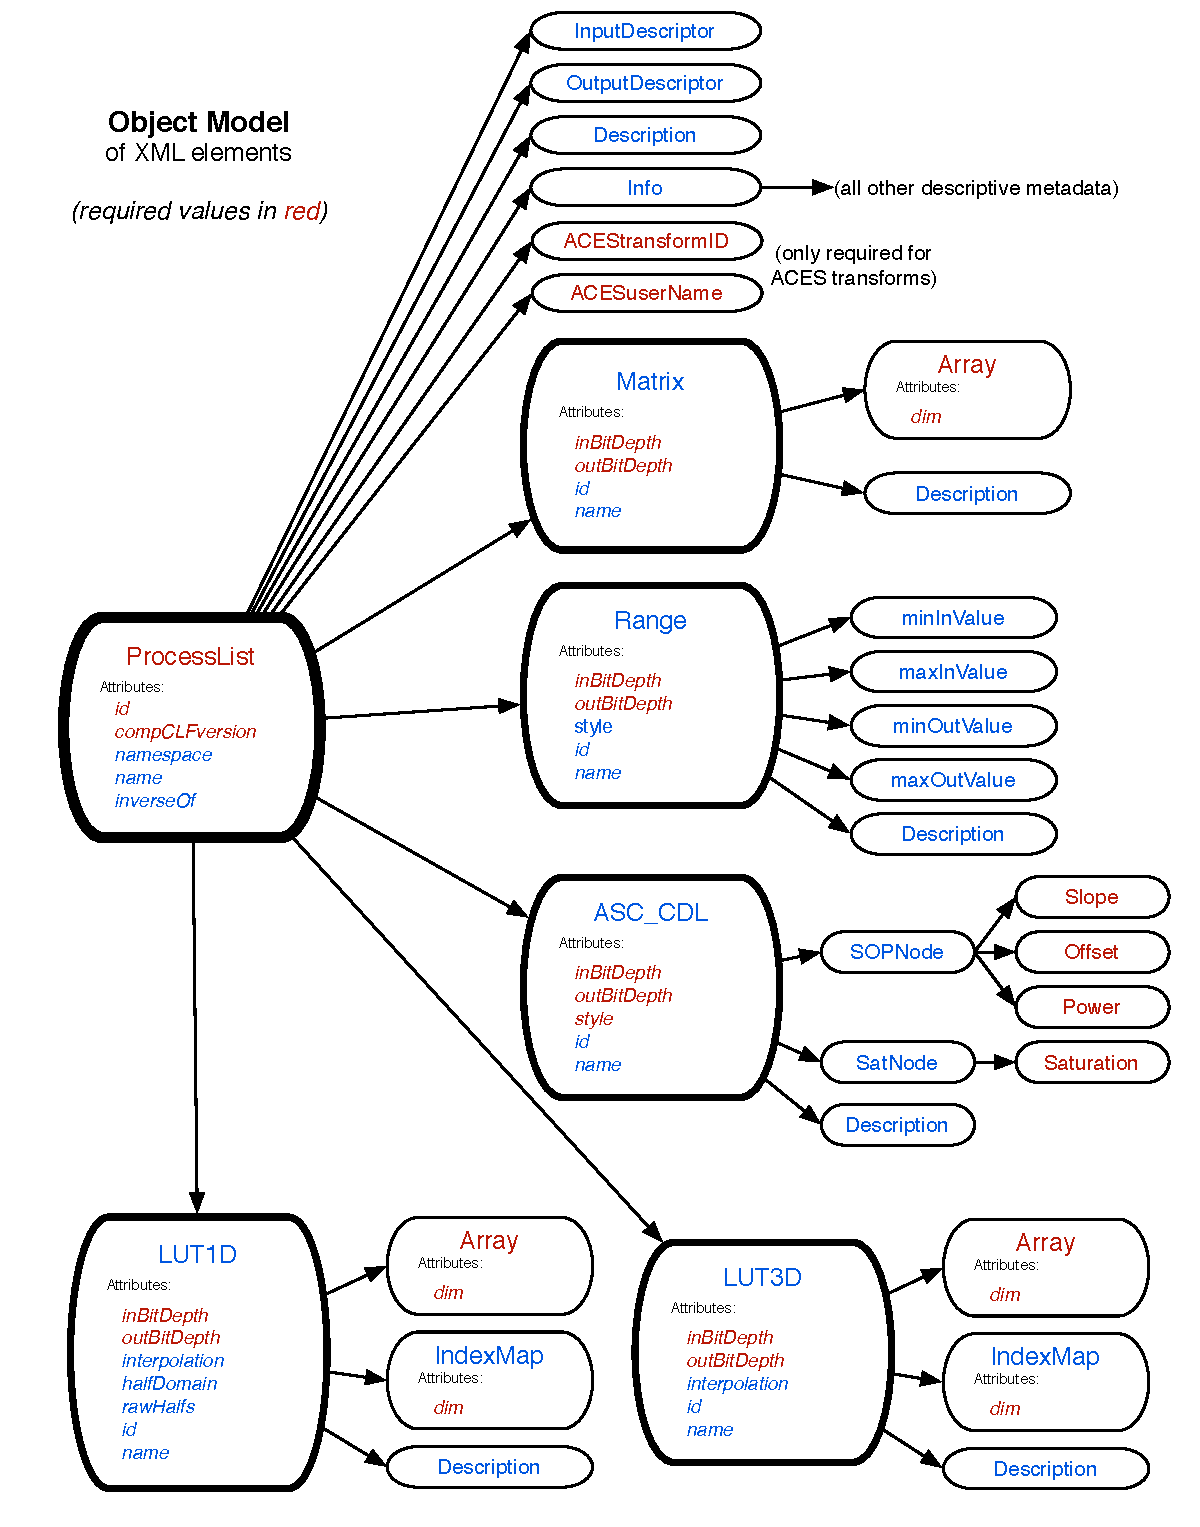
\includegraphics[width=\textwidth]{objectModel.pdf}
\caption{Object Model of XML Elements}
\label{fig:lmt}
\end{center}
\end{figure}
% This file contains the content for a main section
\regularsectionformat
%% Modify below this line %%
\chapter{XML Structure}
\label{sec:XMLstructure}

LUTs are stored in XML files each of which must have the same XML root element, \texttt{ProcessList}, regardless of the number of LUTs in the file. The \texttt{ProcessList} root element contains a sequence of \texttt{ProcessNode}s which are typically either LUTs or matrices. Any \texttt{ProcessList} must also contain at least one \texttt{ProcessNode}. An example of the overall structure of a LUT file is thus:

\lstset{frame=none}
\begin{lstlisting}
<ProcessList id="123">
	<Matrix id="1">
		data & metadata
	</Matrix>
	<LUT1D id="2">
 		data & metadata
	</LUT1D>
	<Matrix id="3">
		data & metadata
	</Matrix>
</ProcessList>	
\end{lstlisting}

The order and number of transforms is determined by the designer of the transform.

The XML file may contain other information that is useful to XML interpreters.  This includes a starting line that identifies the XML version number and Unicode values.  This line is mandatory once in a file and looks like this:

\begin{lstlisting}
<?xml version="1.0" encoding="UTF-8"?>
\end{lstlisting}

The file may also contain XML comments that may be used to describe the structure of the file or save information that would not normally be exposed to a database or to a user.
XML comments are enclosed in brackets like so,     

\begin{lstlisting}
<!--   This is a comment    -->
\end{lstlisting}
\lstset{frame=single}

It is often useful to identify the natural or formal language in which text strings of XML documents are written.  The special attribute named xml:lang may be inserted in XML documents to specify the language used in the contents and attribute values of any element in an XML document. The values of the attribute are language identifiers as defined by IETF RFC 3066. In addition, the empty string may be specified.

The language specified by xml:lang applies to the element where it is specified (including the values of its attributes), and to all elements in its content unless overridden with another instance of xml:lang. In particular, the empty value of xml:lang can be used to override a specification of xml:lang on an enclosing element, without specifying another language.
% This file contains the content for a main section
\regularsectionformat
%% Modify below this line %%
\chapter{XML Elements}
\label{sec:XMLelements}

\section{\texttt{ProcessList}}
This is the root element for any LUT XML file and is required even if only one \texttt{ProcessNode} will be present. A \texttt{ProcessList} is composed of one or more \texttt{ProcessNode}s.

Attributes:
\begin{xmlfields}
	\xmlitem[id][required] Unique identifier of the \texttt{ProcessList}.
	\xmlitem[name][optional] Text name of the \texttt{ProcessList} for display or selection from an application's user interface.
	\xmlitem[compCLFversion][required] Minimum compatible CLF spec version needed to read this file.
	\xmlitem[inverseOf][optional] Optional field for linking to another \texttt{ProcessList id} (unique) which is the inverse of this one.
\end{xmlfields}

Elements:	
\begin{xmlfields}
    \xmlitem[Description][required] Comment field for an arbitrary string describing the function, usage, or notes about the \texttt{ProcessList}. A \texttt{ProcessList} can have one or more \texttt{Description}s.
    \xmlitem[Info][optional] optional element for addition of custom metadata not needed to interpret the transforms. Includes:
    	\begin{xmlfields}
			\xmlitem[AppRelease][optional] application software release level
			\xmlitem[CalibrationInfo][optional] calibration metadata used when making the LUT for a device
			\begin{list}{}{\setlength{\itemsep}{4pt}}
				\item \texttt{\textless DisplayDeviceSerialNum\textgreater}
				\item \texttt{\textless DisplayDeviceHostName\textgreater}
				\item \texttt{\textless OperatorName\textgreater}
				\item \texttt{\textless CalibrationDateTime\textgreater}
				\item \texttt{\textless MeasurementProbe\textgreater}
				\item \texttt{\textless CalibrationSoftwareName\textgreater}
				\item \texttt{\textless CalibrationSoftwareVersion\textgreater}
			\end{list}
    	\end{xmlfields}
    \xmlitem[InputDescriptor][optional] Comment field describing the intended source code values of the \texttt{ProcessList}.
    \xmlitem[OutputDescriptor][optional] Comment field describing the intended output target of the \texttt{ProcessList} (e.g., target display).
    \xmlitem[ProcessNode][required] At least one \texttt{ProcessNode} must be in the list. The \texttt{ProcessNode} is described in \autoref{sec:ProcessNode}.
\end{xmlfields}

\section{\texttt{ProcessNode}}
\label{sec:ProcessNode}
This element represents a process node; it is the primary color transformation element for LUT interchange. Different types of processing are expressed by substitution from this basic element including \texttt{LUT1D}, \texttt{LUT3D}, \texttt{Range} and \texttt{Matrix}. In the future, other kinds of \texttt{ProcessNode}s can be defined as part of the standard to handle alternate forms of processing. All \texttt{ProcessNode} substitutes inherit the attributes and elements below.

Attributes:
\begin{xmlfields}
	\xmlitem[id][optional]  Unique identifier of the \texttt{ProcessNode}.
	\xmlitem[name][optional] Text name of the \texttt{ProcessNode} for display or selection from an application's user interface.
	\xmlitem[inBitDepth][required] Number of bits and type of the input values to which the \texttt{ProcessNode} is applied. The input values can be either integers or floats. Supported values are ``\texttt{8i}'', ``\texttt{10i}'', ``\texttt{12i}'', ``\texttt{16i}'', ``\texttt{16f}'' or ``\texttt{32f}''.
	\xmlitem[outBitDepth][required] Number of bits and type of the output values which the \texttt{ProcessNode} generates. The output values can be either integers or floats, independent of the input values. Supported values are ``\texttt{8i}'', ``\texttt{10i}'', ``\texttt{12i}'', ``\texttt{16i}'', ``\texttt{16f}'' or ``\texttt{32f}''.
\end{xmlfields}

Elements:
\begin{xmlfields}
	\xmlitem[Description][optional] Comment field for an arbitrary string describing the function, usage, or notes about the \texttt{ProcessNode}. A \texttt{ProcessNode} can have one or more \texttt{Description}s.
\end{xmlfields}

\subsection{\texttt{LUT1D} (substitute for \texttt{ProcessNode})}
This element specifies a 1D LUT or a 3by1D LUT.  A 1D LUT transform uses an input pixel value, finds the two nearest index positions in the LUT, and then interpolates the output value using the entries associated with those positions. If the input to a \texttt{LUT1D} is an RGB value, the same LUT will be applied to all three color components. If a 3by1D LUT is supplied, each color component is looked up in a separate \texttt{LUT1D} of the same length. In both cases, the ordered entries of the LUT are provided in \texttt{Array}.  In a 3by1D LUT, by convention, the \texttt{LUT1D} for the first component goes in the first column of \texttt{Array},  etc.).  The lookup operation may be altered by redefining the mapping of the input values to index positions of the LUT using an \texttt{IndexMap}.

Attributes:
\begin{xmlfields}
	\xmlitem[interpolation][optional] Name or description of the preferred calculation used to interpolate values from the \texttt{LUT1D}. This attribute is optional with a default of ``\texttt{linear}'' if the attribute is not present. Systems that utilize LUTs may use different types of interpolation; therefore, this attribute is intended as a guide to an application if it wants to attempt recreating the exact outputs of the originating application. Typical values for this attribute would be ``\texttt{linear}'' or ``\texttt{cubic}''.
	\xmlitem[rawHalfs][optional] If this attribute is present, its value must be ``\texttt{true}''. In this case, the output array values in the form of unsigned 16-bit integers are interpreted as the equivalent bit pattern, half floating-point values. (e.g.  to represent the value 1.0, enter the integer 15360 in the \texttt{Array} element because it has the same bit-pattern. This allows specification of exact half-float values without relying on conversion from decimal text strings.)
	\xmlitem[halfDomain][optional] If this attribute is present, its value must be ``\texttt{true}''. In this case, the input domain to the node is all possible 16-bit floating-point values, and there must be exactly 65536 entries in the LUT1D \texttt{Array} element (e.g. the unsigned integer 15360 has the same bit-pattern (0011110000000000) as the half-float value 1.0, so the 15360th, zero-indexed, entry in the \texttt{Array} element is the output value corresponding to an input value of 1.0). The \texttt{IndexMap} may not be used in this case.
\end{xmlfields}

Elements:
\begin{xmlfields}
	\xmlitem[IndexMap][optional] Table that maps input values to index positions of the \texttt{LUT1D}'s \texttt{Array}.\par
		In its simplest form, with a dim=2, this element can be used to define the input floating-point range that will be used by the LUT.\par
		An extension to the LUT format described in Appendix \ref{appendixC}.
	\xmlitem[Array][required] Table that provides the entries of the \texttt{LUT1D} from the minimum to the maximum input values. In a 3by1D LUT, each column in \texttt{Array} provides the 1D LUT for a color component; for RGB, the 1st column corresponds to R’s 1D LUT, the 2nd column corresponds to G’s 1D LUT, etc.
\end{xmlfields}


\subsection{\texttt{LUT3D} (substitute for \texttt{ProcessNode})}
This element specifies a 3D LUT. In a \texttt{LUT3D} element, the 3 color components of the input value are used to find the nearest indexed values along each axis of the 3D cube. The 3-component output value is calculated by interpolating within the volume defined by the nearest corresponding positions in the LUT. The lookup operation may be altered by redefining the mapping of the input values to index positions into the LUT (see \texttt{IndexMap}). An interpolation comment field is provided to indicate the preferred interpolation calculation to perform within the volume.

Attributes:
\begin{xmlfields}
	\xmlitem[interpolation][optional] Name or description of the preferred calculation used to interpolate values in the \texttt{3DLUT}. This attribute is optional with a default of ``\texttt{trilinear}'' if the attribute is not present. Systems that utilize LUTs may use different types of interpolation; therefore, this attribute is  intended as a guide to an application if it wants to attempt recreating the exact outputs of the originating application. Typical values for this attribute would be ``\texttt{trilinear}'' or ``\texttt{tetrahedral}''.
\end{xmlfields}

Elements:
\begin{xmlfields}
	\xmlitem[IndexMap][optional] Table that maps input values to index positions of the \texttt{LUT3D}'s \texttt{Array}. 
		In its simplest form, with a dim=2, this element can be used to define the input floating-point range that will be used by the LUT.\par
		An extension to the LUT format described in Appendix \ref{appendixC}.
	\xmlitem[Array][required] Table comprised of the entries for the \texttt{LUT3D} from the minimum to the maximum input values, the third component index changing fastest.

		Ex:   order of entries for a 2x2x2 cube by index $[0 \ldots 1]$
		
		\begin{center}
			\begin{tabularx}{1in}{XXX}
				0 & 0 & 0 \\
				0 & 0 & 1 \\
				0 & 1 & 0 \\
				0 & 1 & 1 \\
				1 & 0 & 0 \\
				1 & 0 & 1 \\
				1 & 1 & 0 \\
				1 & 1 & 1 \\
			\end{tabularx}
		\end{center}
\end{xmlfields}

\subsection{\texttt{Matrix} (substitute for \texttt{ProcessNode})}
This element specifies a matrix transformation to be applied to the input values. The input and output of a \texttt{Matrix} are always 3-component values. All matrix calculations should be performed in floating point, and input bit depths of integer type should be treated as scaled floats. If the input bit depth and output bit depth do not match, the coefficients in the matrix must incorporate the results of the `scale' factor that will convert the input bit depth to the output bit depth (e.g. input of \texttt{10i} with an output of \texttt{12i} requires the matrix coefficients already have a factor of 4095/1023 applied). Changing the input or output bit depth requires creation of a new set of coefficients for the LUT.

The output values are calculated using the row-order convention:

\begin{equation}
    \begin{bmatrix*}
        a_{11} & a_{12} & a_{13} \\
        a_{21} & a_{22} & a_{23} \\
        a_{31} & a_{32} & a_{33} \\
    \end{bmatrix*} \\
    \begin{bmatrix}
        r\\
        g\\
        b
    \end{bmatrix}
    =
    \begin{bmatrix}
        R\\
        G\\
        B
    \end{bmatrix}
\end{equation}
\begin{align*}		
	R = (r \cdot a_{11}) + (g \cdot a_{12}) + (b \cdot a_{13}) \\
	G = (r \cdot a_{21}) + (g \cdot a_{22}) + (b \cdot a_{23}) \\
	B = (r \cdot a_{31}) + (g \cdot a_{32}) + (b \cdot a_{33})
\end{align*}

An offset matrix may be defined as a 3x4 array in which the input value is typically defined as ($r$, $g$, $b$, 1.0).  The 4th column of the matrix may then be used to add an offset term to the conversion of the matrix. The output of the 3x4 matrix is ($R$, $G$, $B$). Matrices using an offset calculation will have one more column than rows.

\begin{equation}
    \begin{bmatrix*}
        a_{11} & a_{12} & a_{13} & off1\\
        a_{21} & a_{22} & a_{23} & off2\\
        a_{31} & a_{32} & a_{33} & off3\\
    \end{bmatrix*} \\
    \begin{bmatrix}
        r\\
        g\\
        b\\
        1.0
    \end{bmatrix}
    =
    \begin{bmatrix}
        R\\
        G\\
        B
    \end{bmatrix}
\end{equation}
 
Elements:
\begin{xmlfields}
	\xmlitem[Array][required] Table that provides the coefficients of the transformation matrix. The matrix dimensions are either 3x3 or 3x4. The matrix is serialized row by row from top to bottom and from left to right, i.e., ``$a_{11}\ a_{12}\ a_{13}\ a_{21}\ a_{22}\ a_{23}\ \ldots$'' for a 3x3 matrix.
		\begin{equation}
		    \begin{bmatrix*}
		        a_{11} & a_{12} & a_{13} \\
		        a_{21} & a_{22} & a_{23} \\
		        a_{31} & a_{32} & a_{33} \\
		    \end{bmatrix*} \\
		\end{equation}
	
\end{xmlfields}

\subsection{\texttt{Range} (substitute for \texttt{ProcessNode})}
The \texttt{Range} element maps the input domain to the output range by scaling and offsetting values and must be calculated in floating point. The \texttt{Range} element is also used to clamp values.

If a \texttt{minInValue} is present, then \texttt{minOutValue} must also be present and the result is clamped at the low end. Similarly, if \texttt{maxInValue} is present, then \texttt{maxOutValue} must also be present and the result is clamped at the high end. If none of \texttt{minInValue}, \texttt{minOutValue}, \texttt{maxInValue}, or \texttt{maxOutValue} are present, then the \texttt{Range} operator performs only scaling.

The scaling of \texttt{minInValue} and \texttt{maxInValue} depends on the input bit depth, and the scaling of \texttt{minOutValue} and \texttt{maxOutValue} depends on the output bit depth.

Elements:
\begin{xmlfields}
	\xmlitemopt[minInValue][optional]
	\xmlitemopt[maxInValue][optional]
	\xmlitemopt[minOutValue][optional]
	\xmlitemopt[maxOutValue][optional]
\end{xmlfields}

Attributes:
\begin{xmlfields}
	\xmlitem[style][optional]
		Description of the preferred handling of the scaling calculation of the \texttt{Range} node. If the style attribute is not present, clamping is performed.
		\begin{xmlfields}
			\xmlitemd[``noClamp''] If present, do not apply the clamping in the equations below (i.e. floating point values above \texttt{maxOutValue} are allowed). 
			\xmlitemd[``Clamp''] If present, clamping is applied according to:
				\begin{equation}
					\mathrm{MIN}(\texttt{maxOutValue}, \mathrm{MAX}( \texttt{minOutValue}, RGB_{out} ))
				\end{equation}
		\end{xmlfields}
\end{xmlfields}

The range between \texttt{minInValue} and \texttt{maxInValue} is scaled to the \texttt{minOutValue} and \texttt{maxOutValue} range using the following equation:
\begin{align*}
	scale &= \dfrac{(\texttt{maxOutValue} - \texttt{minOutValue})}{(\texttt{maxInValue} - \texttt{minInValue})} \\
	RGB_{out} &= RGB_{in} \times scale + \texttt{minOutValue} - \texttt{minInValue} \times scale \\
	RGB_{out_{clamped}} &= \mathrm{MIN}(\texttt{maxOutValue}, \mathrm{MAX}( \texttt{minOutValue}, RGB_{out}))
\end{align*}

If the input and output bit depths are not the same, a conversion should take place using the range elements. If the elements defining an \texttt{InValue} range or \texttt{OutValue} range are not provided, then the default behavior is to use the full range available with the \texttt{inBitDepth} or \texttt{outBitDepth} attribute used in place of the missing input range or missing output range, respectively, as calculated with these equations:

In the formulae below, if the bit depth is integral, then rangescalar() is defined as:
	\begin{equation} 
	 	\mathrm{rangescalar}( bitDepthInteger ) = 2^{bitDepth} - 1
	\end{equation}
If the bit depth is specified as floating point, then:
	\begin{equation} 
		\mathrm{rangescalar}( float ) = 1.0
	\end{equation}

If only minimum values are specified, the formula is:
	\begin{align*}
		scale &= \dfrac{\mathrm{rangescalar}(outBitDepth)}{\mathrm{rangescalar}(inBitDepth)} \\
		RGB_{out} &= \mathrm{MAX}( \texttt{minOutValue}, RGB_{in} \times scale + \texttt{minOutValue} - \texttt{minInValue} \times scale)		
	\end{align*}

If only maximum values are specified, the formula is:
	\begin{align*}
		scale &= \dfrac{\mathrm{rangescalar}(outBitDepth)}{\mathrm{rangescalar}(inBitDepth)} \\
		RGB_{out} &= \mathrm{MIN}( \texttt{maxOutValue}, RGB_{in} \times scale + \texttt{maxOutValue} - \texttt{maxInValue} \times scale)		
	\end{align*}

\subsection{\texttt{ASC\_CDL} (substitute for \texttt{ProcessNode})}
This node contains the parameters for processing pixels using the ASC CDL color correction equations. The ASC CDL equations are designed to work on an input domain of floating-point values of [0 to 1.0] although values greater than 1.0 can be present. The output data may or may not be clamped depending on the processing configuration below.

Attributes:
\begin{xmlfields}
	\xmlitem[id][optional] This should match the id attribute of the ColorCorrection element in the ASC CDL XML format.
	\xmlitem[style][optional] Determines the formula applied by the operator. The valid options are:
		\begin{xmlfields}
			\xmlitemd["Fwd"] implementation of v1.2 ASC CDL equation
			\xmlitemd["Rev"] inverse equation
			\xmlitemd["FwdNoClamp"] similar to the \texttt{Fwd} equation, but without clamping
			\xmlitemd["RevNoClamp"] inverse equation
		\end{xmlfields}
		The first two implement the math provided in version 1.2 of the ASC CDL specification.  The second two omit the clamping step and are intended to provide compatibility with the many applications that take that alternative approach.
\end{xmlfields}

Elements:
\begin{xmlfields}
	\xmlitem[SOPNode][optional] The \texttt{SOPNode} is optional, but if present, must contain one each of the following sub-elements:
	\begin{xmlfields}
		\xmlitemd[Slope] If not provided, the default is 1.0 for all channels.
		\xmlitemd[Offset] If not provided, the default is 0.0 for all channels.
		\xmlitemd[Power] If not provided, the default is 1.0 for all channels.
	\end{xmlfields}
	\xmlitem[SatNode][optional] The \texttt{SatNode} is optional, but if present, must contain one of the following sub-element:
	\begin{xmlfields}
		\xmlitemd[Saturation] If not provided, the default is 1.0 for all channels.
	\end{xmlfields}
\end{xmlfields}

\note{The structure of this \texttt{ProcessNode} matches the structure of the XML format described in the v1.2 ASC CDL specification. However, unlike the ASC CDL XML format, there are no alternate spellings allowed for these elements.}

The math for \texttt{style="Fwd"} is:
	\begin{align*}
		SAT_{in} &= \mathrm{clamp}(RGB_{in} \times slope + offset)^{power} \\
		luma &= 0.2126 * SAT_{in_R} + 0.7152 * SAT_{in_G} + 0.0722 * SAT_{in_B} \\
		RGB_{out} &= \mathrm{clamp}(luma + saturation * (SAT_{in} - luma))
	\end{align*}

where clamp() clamps the argument to [0,1].

The math for \texttt{style="FwdNoClamp"} is the same as for \texttt{"Fwd"} but the two clamp() functions are omitted. Also, if $(input * slope + offset) < 0$, then no power function is applied.

The math for \texttt{style="Rev"} is:
	\begin{align*}
		RGB_{in_{clamp}} &= \mathrm{clamp}(RGB_{in}) \\
		luma &= 0.2126 * R_{in_{clamp}} + 0.7152 * G_{in_{clamp}} + 0.0722 * B_{in_{clamp}} \\
		RGB_{sat_{out}} &= luma + \frac{1}{saturation} * (RGB_{in_{clamp}} - luma) \\
		RGB_{out} &= \mathrm{clamp}\left(\frac{\mathrm{clamp}(RGB_{sat_{out}})^{\frac{1}{power}} - offset}{slope}\right) \\
	\end{align*}

The math for \texttt{style="RevNoClamp"} is the same as for \texttt{"Rev"} but the two clamp() functions are omitted. Also, if $RGB_{sat_{out}} < 0$, then no power function is applied.

\note{The equations above assume that the input and output bit depths are floating-point. For integer inputs and outputs, the values must be normalized to or from [0.0, 1.0] scaling. In other words, the slope, offset, power, and saturation values stored in the \texttt{ProcessNode} do not depend on \texttt{inBitDepth} and \texttt{outBitDepth} they are always interpreted as if the bit depths were float.}


\section{\texttt{IndexMap} element} \label{sec:indexmap}
This element defines a list that is a new mapping of input code values, $inValues$, to index positions, $n$, in a LUT's \texttt{Array}. The format of each item in the list is $newInValue\mathrm{@}n$. For example, the first \texttt{IndexMap} item might be $64\mathrm{@}0$ which assigns the $inValue=64.0$ to position $0$ in the LUT. 

In its simplest form, with a \texttt{dim=2}, this element can be used to define the input floating point range that will be used by the LUT.

An extension to the LUT format described in Appendix \ref{appendixC}.

Attributes:
\begin{xmlfields}
	\xmlitem[dim][required] Field that specifies the number of items in the list.	
\end{xmlfields}

\section{\texttt{Array} element}
This element contains the table entries of a LUT in order from minimum value to maximum value with a single line for each color component triple.  The \texttt{dim} attribute specifies the dimensions of the cube, the length of the LUT, or the size of the array.

The \texttt{dim} attribute and the type of node should match.

Attributes:
\begin{xmlfields}
	\xmlitem[dim][required] 	Specifies the dimension of the LUT or the matrix and the number of components. The data points for a \texttt{ProcessNode} are contained in an XML array element. The \texttt{dim} attribute provides the dimensionality of the indexes, where:

		4 entries have the dimensions of a 3D cube plus the number of components per entry.
		\begin{list}{}{\setlength{\itemsep}{4pt}\setlength{\topsep}{0pt}}
				\item e.g. \texttt{dim = 17 17 17 3 } indicates a 17-cubed 3D lookup table with 3 component color
		\end{list}

		3 entries have the matrix dimensions and component value.
		\begin{list}{}{\setlength{\itemsep}{4pt}\setlength{\topsep}{0pt}}
				\item e.g. \texttt{dim = 3 3 3 } is a 3 by 3 matrix acting on 3-component values
				\item e.g. \texttt{dim = 3 4 3 } is a 3 by 4 matrix acting on 3-component values
		\end{list}

		2 entries have the length of the LUT and the component value (1 or 3).
		\begin{list}{}{\setlength{\itemsep}{4pt}\setlength{\topsep}{0pt}}
				\item e.g. \texttt{dim = 256 3 } indicates a 256 element 1D LUT with 3 components (a 3by1DLUT)
				\item e.g. \texttt{dim = 256 1 } indicates a 256 element 1D LUT with 1 component (1DLUT)
		\end{list}
\end{xmlfields}

% This file contains the content for a main section
\regularsectionformat
%% Modify below this line %%
\chapter{Examples}
\label{sec:examples}

This section illustrates some of the typical forms of the LUT format. It should be noted that these are not real examples.

The simplest form is an XML file containing a single node:

\begin{lstlisting}[caption=Example of a ``LUT1D'']
<?xml version="1.0" encoding="UTF-8"?>
<ProcessList xmlns="urn:NATAS:ASC:LUT:v1.2" id="ex1" name="example 1 transform">
	<Description> Turn 4 grey levels into 4 inverted codes using a 1D </Description>
	<LUT1D id="lut-23" name="4valueLut" inBitDepth="12i" outBitDepth="12i">
		<Description> 1D LUT </Description>
		<Array dim="4 1">
			3
			2
			1
			0
		</Array>
	</LUT1D>
</ProcessList>
\end{lstlisting}

The \texttt{LUT1D} ProcessNode could be replaced with a 3D LUT (\autoref{ex:3dlut}) or a matrix (\autoref{ex:matrix}).

\begin{lstlisting}[caption=Example of a \texttt{LUT3D},label=ex:3dlut]
<LUT3D id="lut-24" name="green look" interpolation="trilinear" 
	inBitDepth="12i" outBitDepth="16f">
	<Description> 3D LUT </Description>
	<Array dim="2 2 2 3">
		0.0 0.0 0.0
		0.0 0.0 1.0
		0.0 1.0 0.0
		0.0 1.0 1.0
		1.0 0.0 0.0
		1.0 0.0 1.0
		1.0 1.0 0.0
		1.0 1.0 1.0
	</Array>
</LUT3D>

\end{lstlisting}

\begin{lstlisting}[caption=Example of a \texttt{Matrix},label=ex:matrix]
<Matrix id="lut-25" name="colorspace conversion" inBitDepth="10i" outBitDepth="10i" >
	<Description> 3x4 Matrix , 4th column is offset </Description>
	<Array dim="3 4 3">
		1.2  	0.0  	0.0   	0.002
		0.0 	1.03 	0.001 	-0.005
		0.004 	-0.007 	1.004  	0.0
	</Array>
</Matrix>

\end{lstlisting}

``Shaper LUTs'' require a bit more of an explanation.  This is once again an illustration of the technique using an \texttt{IndexMap} and not a real world example. These can also be implemented with \texttt{1DLUT}s.

\begin{lstlisting}[caption=Example of a partially enumerated ``Shaper LUT'',label=ex:shaperlut]
<LUT1D id="lut-25" name="shaper LUT" inBitDepth="10i" outBitDepth="16f">
	<Description> 1D LUT with shaper </Description>
	<IndexMap dim=4>0@0 10@100 20@250 30@360 40@440 445@445 
					700@600 800@700 900@850 950@1023</IndexMap>
	<Array dim="1024 1">
		0.00
		0.32
		0.50
		<1020 entries omitted>
		1.0
	</Array>
</LUT1D>
\end{lstlisting}

\begin{lstlisting}[caption=Example of an ASC CDL node,label=ex:asccdl]
<ASC_CDL id="cc01234" inBitDepth="16f" outBitDepth="16f" style="Fwd">
	<Description>scene 1 exterior look</Description>
	<SOPNode>
		<Slope>1.000000  1.000000  0.900000</Slope>
		<Offset>-0.030000  -0.020000  0.000000</Offset>
		<Power>1.2500000  1.000000  1.000000</Power>
	</SOPNode>
	<SatNode>
		<Saturation>1.700000</Saturation>
	</SatNode>
</ASC_CDL>

\end{lstlisting}

A full example of an XML file (\autoref{ex:fullexample}) shows three nodes in a ProcessList.

\begin{lstlisting}[caption=Full example of an XML LUT file,label=ex:fullexample]
<?xml version="1.0" encoding="UTF-8"?>
<ProcessList xmlns="urn:NATAS:ASC:LUT:v1.2" id="luts-23+24+25" name="lut chain 34">
	<Description> Turn 4 grey levels into 4 codes for a monitor using a 3by1D LUT 
			into 3D LUT into 3x1D LUT </Description>
	<OutputDescriptor> Sony BVM CRT </OutputDescriptor>
	<LUT1D id="lut-23" name="input lut" inBitDepth="12i" outBitDepth="12i">
		<Description> 3by1D LUT </Description>
		<Array dim="4 3">
			1 1 1
			1 1 1
			2 2 2 
			2 2 2
		</Array>
	</LUT1D>
	<LUT3D id="lut-24" name="green look output rendering" interpolation="trilinear"
				inBitDepth="12i" outBitDepth="16f">
		<Description> 3D LUT </Description>
		<Array dim="4 4 4 3">
			0.0 0.0 0.0
			0.0 0.0 1.0
			0.0 1.0 0.0
			0.0 1.0 1.0
			1.0 0.0 0.0
			1.0 0.0 1.0
			1.0 1.0 0.0
			1.0 1.0 1.0
			[ed:  ...abridged:   64 total entries...]
			1.0 1.0 1.0
		</Array>
	</LUT3D>
	<LUT1D id="lut-25" name="output conversion" inBitDepth="16f" outBitDepth="12i">
		<Description> 3x1D LUT </Description>
		<IndexMap dim=2>0.0@0 3.0@65504.0</IndexMap>
		<Array dim="4 3">
			0 0 0 
			1 1 1
			2 2 2 
			3 3 3
		</Array>
	</LUT1D>
</ProcessList>

\end{lstlisting}

% This file contains the content for a main section
\regularsectionformat
%% Modify below this line %%
\chapter{Implementation Notes}
\label{sec:implementation}

\section{Efficient Processing}
The transform engine may merge some or all of the transforms and must maintain appropriate precision in the calculations so that output values are correct. It is recommended that all calculations be done in at least 32-bit floating point. High accuracy for 16-bit half float output is required.

The existence of a common LUT format cannot guarantee that the resulting images will look the same on all implementations as numerical accuracy issues in implementations can have a significant effect on image appearance.

The engine may create a single LUT concatenating the output result of all of the node calculations but this may introduce some inaccuracies to the result due to LUT sampling errors. It is up to the user to determine whether these approximate results are sufficient.  

\section{Indexing Calculations}
A \texttt{ProcessNode} using LUT tables must perform an index calculation to take the range of input values and ratio them to the input `index' range of the table (i.e. the minimum and maximum index positions into the table). This allows the LUT location calculation to be easily achieved as the normalized index function can be multiplied by the number of entries in the LUT to get a direct hash function to the appropriate LUT locations. For integer inputs, this is straightforward as the \texttt{inBitDepth} attribute may be used to apply the whole range of input across the whole range of index positions.

\section{Floating-point Output of the \texttt{ProcessList}}
The output of the LUT chain should be intended for real devices, therefore a transform designer and/or the application should insure that output floating-point values do not contain infinities and NaN codes. The minimum and maximum representable integer values should be used instead. It is the responsibility of the application to handle overflows and underflows correctly.

In most applications, it is either the internal requirements of the application or the end-user who controls the bit depth of pixels being processed through a \texttt{ProcessList}. So transform authors should not assume that applications will necessarily clamp and quantize based on the settings of the \texttt{outBitDepth} attribute for the last node of the \texttt{ProcessList}.

\textit{Floating-point processing:}

Although it has been traditional practice in converting from integer to floats to normalize the top integer code to a value of 1.0 in floating point, there is an increasing need for calculations in high-dynamic range imaging systems where this assumption might be flawed, so the assumption in the \texttt{ProcessList} element is that integer values are normalized floats where for example of 1023 in integer is output from a node as 1.0. A \texttt{Range} node is provided to make explicit the choice of scaling that a LUT designer wants to provide in his transform, including the normalization step. Floating-point values may exceed this range, but LUTs designed for output devices should also aim towards a final normalized result compatible with the integer range.

\section{Half-float 1DLUTs}
When the input to a \texttt{LUT1D} is 16f, the \texttt{halfDomain} attribute may be used to indicate that the value to be used for the lookup into the array treats the 16f value as an integer. As an example, the half-float value 1.0 will be the 15360th (zero-indexed) entry in the array. The simplest implementation of this requires that the LUT1D thus be fully enumerated with 65536 entries. The design of this 1D array must take into account the presence of negative numbers, infinities, and NaNs in the original 16f bit pattern.

(code values 31744-32767 and 64513-65535 are infinity or NaNs)

Similarly, the \texttt{rawHalf} attribute may be used to indicate that the integer 16 bit output values in each position of the output array represent the bit-equivalent, half floating-point values.  

The floating-point values input to a node may have been manipulated via a \texttt{Range} node which may clamp values to a specific smaller range of floating-point values (the values of 0.0 to 1.0 being a common choice).  

\section{Rescaling operations for input and output to a \texttt{ProcessNode}}
The input and output bit depths of a single node may not match each other. For 1DLUTs and 3DLUTs, the output array values are assumed to be in the output bit depth. For \texttt{Matrix} elements, a scale factor must be applied within the coefficients of the matrix.

\section{Rescaling operations for input and output to a \texttt{ProcessList}}
There are scenarios where applications must change the input and output bit depth (\texttt{inBitDepth} and \texttt{outBitDepth}, respectively) of a \texttt{ProcessList}. One scenario is when the pixels supplied to or returned, when applying a transform, do not match the bit depth used by the transform creator. Another scenario is when combining two \texttt{ProcessList}s.  When changing or converting float to integer bit depths, a scale factor of $2^N-1$ is applied. The inverse scale factor is applied when converting integer to float.  Conversions between differing integer bit depths may be derived from these scale factors.

\section{Type conversion between integer and float}
Conversions from float to integer if required must be done by rounding. The output bit depth does not require that any node convert and quantize to integer values. The decision to quantize is made by the application invoking the \texttt{ProcessList}.

Conversions from integers with bit depth $n$ to float should be done by:

$floatValue =  \dfrac{intValue}{(2^n-1)}$

\section{Interpolation Types}
When an interpolation type is not listed, it is usually assumed to be linear interpolation (see example in definitions under “Sampled LUT”) or tri-linear in the case of a 3DLUT. Applications must support tetrahedral interpolation for 3DLUTs.

A comment field is provided to identify the type of interpolation used for a particular cube. In many cases, the details of an interpolation used within a product may not be available. The interpolation type field is currently only a hint. Therefore, there is no assurance that images processed with the same XML LUT file on different hardware or software systems will yield the same resulting image. At the moment, this problem is outside the scope of the committee’s work. Hopefully, details on interpolations will be published or become more widely available in the future. Further, a common reference implementation of the LUT format may be able to achieve some standardization of common interpolation types.
 
\section{XML File White Space}
It is desirable that the \texttt{Array} elements keep single lines per entry so that a file can quickly be scanned by a human reader. There are some difficulties with this though as XML has some non-specific methods for handling white-space and thus if files are re-written from an XML parser, exact white spacing is not necessarily maintained. XML style sheets may be used for reviewing and checking the LUT's entries to keep the line layout the same.

There is also the issue that is known to exist between Mac, Unix, and PC text files that have differing end-of-line conventions \textless{}CR\textgreater{}\textless{}LF\textgreater{} vs. \textless{}CR\textgreater{}. This may cause collapse of the values into one long line. The `newline' string, i.e. the byte(s) to be interpreted as ending each line of text, is the single code value $10_{10} = 0\mathrm{A}_{16}$ (ASCII `Line Feed' character), also indicated \textless{}lf\textgreater{}; this newline convention for text files is native to all *nix operating systems (including Linux and current Apple OSs).

In addition to the above, parsers for this file format can be allowed to interpret either Microsoft's \textless{}cr\textgreater{}\textless{}lf\textgreater{} or old-style MacOS' \textless{}cr\textgreater{} newline conventions, but they should not generate CommonLUT files with this encoding.

\section{Extensions}
It is recommended that if readers find an unrecognized element outside of the \texttt{Info} block that they either raise an error or at least provide a warning message to the user. This could be an indication that there is a \texttt{ProcessNode} that is not recognized by the reader.

The \texttt{Info} block in the \texttt{ProcessList} should be used for custom metadata that is unlikely to be recognized by other applications.
% This file contains the content for a main section
\regularsectionformat
%% Modify below this line %%
\chapter{Conclusions}
\label{sec:conclusions}

The XML format provides an extensible and straightforward method for exchanging LUT and matrix data between users and facilities. New types of \texttt{ProcessNode}s can be defined in the future to handle other desired forms of color processing. Among possible additions are nodes that provide  CTL (Color Transformation Language) processing or custom formula transforms such as the ACES RRT.

Feedback from users and from implementers may lead to changes in the specification or schema, so readers should verify usage of the latest version of this document. At this time, there is no reference implementation available for distribution.

The Academy/ASC Common LUT Format is a powerful tool for handling the exchange of LUTs and color transformations between facilities.  It has the potential to become an archival element that would be as useful to the industry as the paper tape timing lights still found today in film cans.

\begin{appendices}
    \appendixchapter{Encoding of negative values}{i}
\label{appendixA}

Very small ACES scene referred values below $7\,^1/_4$ stops below 18\% middle gray are encoded as negative ACEScc values. These values should be preserved per the encoding in \autoref{sec:ACEScc} so that all positive ACES values are maintained.

When ACES values are matrixed into the smaller ACEScc color space, colors outside the ACEScc gamut can generate negative values even before the log encoding. If these values are clipped, a conversion back to ACES will not restore the original colors. A specific method of preserving negative values produced by the transformation matrix has not been defined in part to help ease adoption across various color grading systems that have different capabilities and methods for handling negative values. Clipping these values has been found to have minimal visual impact when viewed through the Reference Rendering Transform (RRT) and an appropriate Output Device Transform (ODT) on currently available display technology. However to preserve creative choice in downstream processing and to provide the highest quality archival master, developers implementing ACEScc encoding are encouraged to adopt a method of preserving negative values so that a conversion from ACES to ACEScc and back can be made lossless. Alternatively, a gamut mapping algorithm may be applied to minimize hue shifts resulting from clipping negative ACEScc values. Specific methods for handling negative values may be added to the ACEScc specification in the future.
    \appendixchapter{Application of ASC CDL parameters to ACEScc image data}{i}
\label{appendixB}

American Society of Cinematographers Color Decision List (ASC CDL) slope, offset, power, and saturation modifiers can be applied directly to ACEScc image data. ASC CDL color grades created on-set with ACESproxy images per the ACESproxy specification will reproduce the same look when applied to ACEScc images. ACEScc images however aren’t limited to the ACESproxy range. To preserve the extended range of ACEScc values, no limiting function should be applied with ASC CDL parameters. The power function, however, should not be applied to any negative ACEScc values after slope and offset are applied. Slope, offset, and power are applied with the following function.

\begin{gather*} 
    ACEScc_{out} = \left\{ 
    \begin{array}{l r }
        ACEScc_{in} \times slope + offset; & \quad ACEScc_{slopeoffset} \leq 0 \\
        (ACEScc_{in} \times slope + offset)^{power}; & \quad ACEScc_{slopeoffset} > 0 \\
    \end{array} \right. \\ 
    \\
    \begin{array}{l}
    \text{Where:}\\
    ACEScc_{slopeoffset} = ACEScc_{in} \times slope + offset
    \end{array}
\end{gather*}

ASC CDL Saturation is also applied with no limiting function:

\begin{gather*}
    luma = 0.2126 \times ACEScc_{red} + 0.7152 \times ACEScc_{green} + 0.0722 \times ACEScc_{blue} \\
    \begin{aligned}
        ACEScc_{red} &= luma + saturation \times (ACEScc_{red} - luma) \\
        ACEScc_{green} &= luma + saturation \times (ACEScc_{green} - luma) \\        
        ACEScc_{blue} &= luma + saturation \times (ACEScc_{blue} - luma) \\ 
    \end{aligned}
\end{gather*}
    
    \appendixchapter{Convention for use of ACESproxy SMPTE range}{i}
\label{appendixC}

This appendix defines the equivalent of a [0.0 \ldots{} 1.0] range in both 10-bit and 12-bit ACESproxy for use in applications.

For consistency in using ACESproxy values in video systems designed around the [0.0 \ldots{} 1.0] video range (encoded in 10-bit video as the range 64-940), the following ACES values are considered the equivalents to 0.0 and 1.0 for both 10-bit and 12-bit video.


\begin{center}
\begin{tabularx}{0.75\textwidth}{|Y|c|c|c|c|}
\hline
\textbf{Video normalized scale} & \textbf{IRE} & \textbf{10-bit CV} & \textbf{12-bit CV} & \textbf{ACES} \\ \hline
0.0 & 0\% & 64 & 256 & 0.001185417 \\ \hline
1.0 & 100\% & 940 & 3760 & 222.875 \\ \hline
\end{tabularx}
\end{center}

ASC CDL values are applied to values in the range [0.0 \ldots{} 1.0] which by this convention are set to ACES values 0.001185417 to 222.875. In integer based color grading systems this is typically accomplished by scaling from ``legal'' to full range before applying ASC CDL transforms. The ASC CDL application is further defined in a separate document.
    \appendixchapter{ACESproxy function derivation}{i}
\label{appendixD}

The ACESproxy 10-bit and 12-bit logarithmic encoding and decoding functions have been derived from the single mathematical function described below. A series of parameters are defined and the values for the parameters specified based on the bit depth of the encoding.

\unnumberedformat
\section{Math functions}
The following general-use math functions are defined for use within the equations.

ROUND$(\mathbf{a})$ \tabto{7em}Math function taking a floating-point value $\mathbf{a}$, and returning the integer value closest to $\mathbf{a}$.

MAX$(\mathbf{a,b})$ \tabto{7em}Math function returning the greater of $\mathbf{a}$ or $\mathbf{b}$

MIN$(\mathbf{a,b})$ \tabto{7em}Math function returning the lesser of $\mathbf{a}$ or $\mathbf{b}$

FLOAT2CV$(\mathbf{a})$ \tabto{7em}Math function returning MAX($CVmin$, MIN($CVmax$, ROUND($\mathbf{a}$)))

\section{Parameters}
The following parameters are defined for each bit-depth.

\begin{itemize}
	\item $CVmin$ is the minimum code value available for representation of ACES image data.
	\item $CVmax$ is the maximum code value available for representation of ACES image data.
	\item $StepsPerStop$ is the number of code values representing a change of 1 stop in exposure.
	\item $MidCVoffset$ is the integer code value representing the assigned midpoint of the exposure scale for a particular bit-depth encoding. (e.g. the point to which a mid-grey exposure value would be mapped)
	\item $MidLogOffset$ is the base 2 logarithmic value representing the assigned midpoint of the exposure scale in log space, [e.g. $MidLogOffset = \log_2( 2^{-2.5} ) = -2.5$ ]
\end{itemize}

\begin{center}
\begin{tabularx}{0.75\textwidth}{|l|Y|Y|}
\hline
	 & \textbf{ACESproxy 10-bit CV} & \textbf{ACESproxy 12-bit CV} \\ \hline
	$CVmin$ & 64 & 256 \\ \hline
	$CVmax$ & 940& 3760 \\ \hline
	$StepsPerStop$ & 50 & 200 \\ \hline
	$MidCVoffset$ & 425 & 1700 \\ \hline
	$MidLogOffset$ & -2.5 & -2.5 \\ \hline
\end{tabularx}
\end{center}

\note{$MidCVoffset$ is not equal to the ACESproxy value that most closely represents an ACES mid-gray value of 0.18. ACES 0.18 is most closely represented by ACESproxy 426 10-bit CV and 1705 12-bit CV.}
 
\newpage
\section{Encoding Function}
The following floating-point equation is used to convert linear values to integer code values.
\begin{equation} 
    \resizebox{\textwidth}{!}{$
    ACESproxy = \left\{ 
    \begin{array}{l l}
        CVmin;    & lin \leq 2^{\left({\frac{(CVmin-MidCVoffset)}{StepsPerStop}-MidLogOffset}\right)} \\
        \mathrm{FLOAT2CV}\left[\left(\log_2(lin)-MidLogOffset\right)\times StepsPerStop+MidCVOffset\right];        & lin > 2^{\left({\frac{(CVmin-MidCVoffset)}{StepsPerStop}-MidLogOffset}\right)} \\
    \end{array} \right. $ }
\end{equation}

where $ACESproxy$ is the resulting integer code value in the range of code values from $CVmin$ to $CVmax$. 


An implementation may use mathematically equivalent forms of this encoding equation.


\section{Decoding Function}
The following floating-point equation is used to convert ACESproxy integer code values to linear values.

\begin{center}
$lin = 2^{\left( \dfrac{(ACESproxy-MidCVoffset)}{StepsPerStop} + MidLogOffset\right)}$

\end{center}

The conversion to linear creates the closest value in 16-bit half precision floating-point to the floating-point result of the equation. Linear values resulting from this equation are limited to the range of values that can be encoded in ACESproxy as illustrated in Appendix \ref{appendixB}. This decoding function does not produce negative values.


An implementation may use mathematically equivalent forms of this decoding equation.
\end{appendices}

\end{document}
